\chapter{विद्युत-रासायनिक सेलों की ऊष्मागतिकी}\label{ch:b2:cell-thermodynamics}

हाइड्रोजन ईंधन-सेल बस कुछ सौ पतले सेलों का एक पुंज ले चलती है। हर एक में
हाइड्रोजन और वायु की ऑक्सीजन बिना ज्वाला के मिलकर जल बनाती हैं, और
ऊर्जा विद्युत धारा के रूप में निकलती है। ऐसे पुंज को दो संख्याएँ नियंत्रित करती हैं, और
दोनों सीधे गिब्स ऊर्जाओं की सारणियों से आती हैं: कोई सेल
\qty{1.23}{V} से अधिक नहीं दे सकता, और कोई ईंधन सेल, चाहे जितना पूर्ण हो, अपनी
हाइड्रोजन की सारी ऊर्जा को विद्युत कार्य में नहीं बदलता। यह अध्याय सेल की वोल्टता को
उसकी अभिक्रिया की \omterm{def:b2:reaction-free-energy:gibbs-energy}{गिब्स ऊर्जा} से जोड़ता है, प्रथम वर्ष के खंड से प्रयुक्त
नेर्न्स्ट समीकरण व्युत्पन्न करता है, और अभिक्रिया की एन्ट्रॉपियाँ और एन्थैल्पियाँ एक वोल्टमापी
और एक तापमापी से पढ़ता है।

\begin{recall}
प्रथम वर्ष का खंड: सेल, अर्ध-सेल, ऐनोड और कैथोड, लवण सेतु, सेल
वोल्टता, इलेक्ट्रोड विभव, मानक विभव और मानक हाइड्रोजन
इलेक्ट्रोड, नेर्न्स्ट समीकरण (वहाँ स्वीकार किया गया), विभवों से साम्य
स्थिरांक। \Cref{ch:b2:reaction-free-energy}: $\Delta_r G$, $\Delta_r G^\circ$
और $\Delta_r G = \Delta_r G^\circ + RT\ln Q$; विकास निकष।
\Cref{ch:b2:chemical-potential}: सक्रियताएँ। विद्यालय का खंड: विद्युत-अपघटन।
\end{recall}

\begin{omfigure}
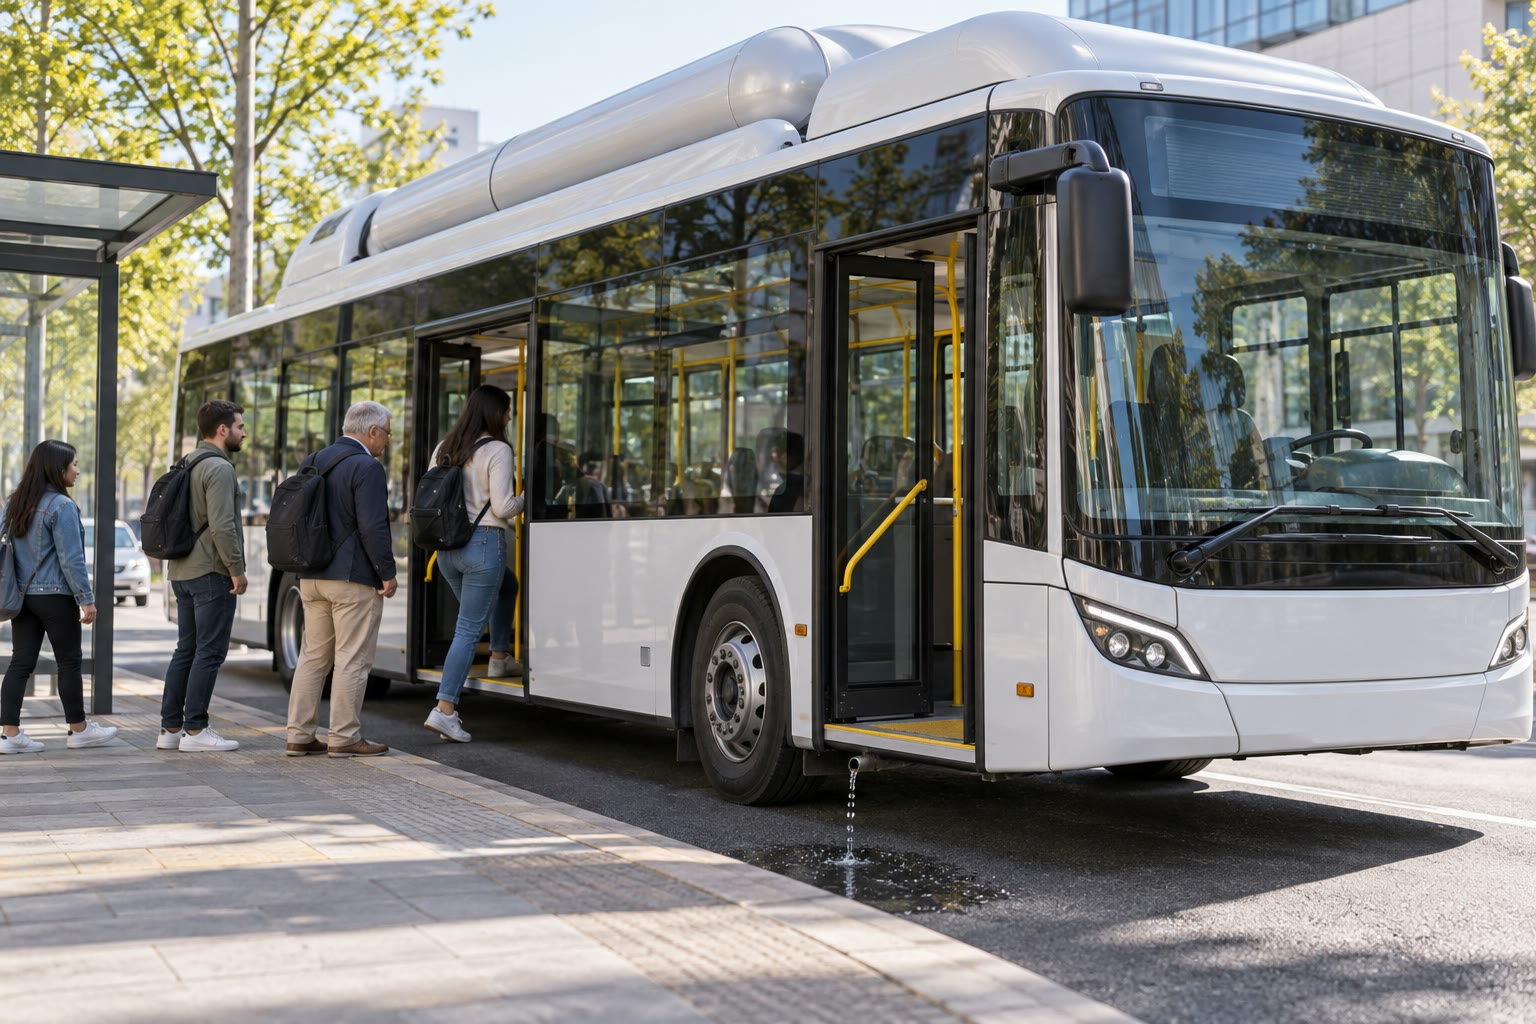
\includegraphics[width=0.62\linewidth]{images/book3/ai/b2-09-fuel-cell-bus.jpg}

{\small पड़ाव पर एक हाइड्रोजन ईंधन-सेल बस: हाइड्रोजन टंकियाँ छत पर आवरण के
नीचे हैं, और एकमात्र निकास जल है, जो बस के नीचे टपकता है।}
\end{omfigure}

\section{विद्युत कार्य और फ़ैराडे स्थिरांक}

\begin{definition}[फ़ैराडे स्थिरांक]\label{def:b2:cell-thermodynamics:faraday}
\emph{फ़ैराडे स्थिरांक}\index{फ़ैराडे स्थिरांक} प्रारंभिक आवेशों के एक मोल का
विद्युत आवेश है, $F = N_A e = \qty{96485.33}{C/mol}$।
% ledger: const:F
\end{definition}

\begin{proposition}[प्रवाहित आवेश]\label{prop:b2:cell-thermodynamics:charge}
यदि $n$ विनिमित इलेक्ट्रॉनों के साथ लिखी गई सेल की अभिक्रिया
$\Delta\xi$ आगे बढ़ती है, तो बाह्य परिपथ से प्रवाहित आवेश $Q =
nF\,\Delta\xi$ है।
\end{proposition}

\begin{proof}
प्रगति $\Delta\xi$ इलेक्ट्रॉनों के $n\,\Delta\xi$ मोल को तार से होकर
ऐनोड से कैथोड तक ले जाती है, हर एक का आवेश परिमाण में $e$:
$Q = n\,\Delta\xi\,N_A e$।
\end{proof}

जब कोई आवेश $Q$ वोल्टता $U$ द्वारा किसी परिपथ से धकेला जाता है, तो परिपथ द्वारा
प्राप्त कार्य $QU$ है। सेल की ओर से देखने पर, जो वह कार्य देता है,
उसके द्वारा प्राप्त विद्युत कार्य $\delta W_{\text{विद्युत}} = -U\,\delta Q = -nFU\,
d\xi$ है।

\begin{omfigure}
\begin{tikzpicture}[font=\small, >={Stealth}]
  \draw[thick, rounded corners, fill=omDef!8] (0,0) rectangle (3.2,2.2);
  \node[align=center] at (1.6,1.1) {सेल\\ (निकाय)\\ अभिक्रिया $d\xi$};
  \draw[->, thick, omThm] (3.2,1.6) -- (5.6,1.6) node[right, align=left] {दिया गया $\delta W_{\text{विद्युत}}$\\ $= nFU\,d\xi$};
  \draw[->, thick, omDef] (5.6,0.6) -- (3.2,0.6) node[pos=0, right, align=left] {प्राप्त $\delta Q_{\text{ऊष्मा}}$\\ (चिह्न कोई भी)};
  \draw[<->, thick] (1.6,2.2) -- (1.6,3.0) node[above] {$T$, $p$ पर परिवेश};
\end{tikzpicture}

{\small नियत ताप और दाब पर ऊष्मागतिक निकाय के रूप में एक सेल:
यह परिवेश से ऊष्मा का विनिमय करता है और बाह्य परिपथ से विद्युत कार्य
देता है। प्रथम नियम की चिह्न परिपाटी के साथ (प्राप्त कार्य और ऊष्मा
धनात्मक गिने जाते हैं), $\delta W_{\text{विद्युत}} = -nFU\,d\xi$।}
\end{omfigure}

\section{सेल अभिक्रिया की गिब्स ऊर्जा}

\begin{theorem}[विद्युत कार्य और गिब्स ऊर्जा]\label{thm:b2:cell-thermodynamics:delta-g-nfe}
नियत $T$ और $p$ पर काम करता सेल अधिक से अधिक अपनी \omterm{def:b2:reaction-free-energy:gibbs-energy}{गिब्स ऊर्जा} की कमी के बराबर
विद्युत कार्य देता है: प्रगति $d\xi$ के लिए
$nFU\,d\xi \leq -\Delta_r G\,d\xi$। जब वह उत्क्रमणीय रूप से (अतिसूक्ष्म
धारा के साथ) काम करता है, तो समता लागू होती है, और सेल वोल्टता
विद्युत-वाहक बल होती है:
\[
  \Delta_r G = -nFE .
\]
\end{theorem}

\begin{proof}
नियत दाब पर प्रथम नियम, दाब-कार्य को अलग करके:
$dH = \delta Q + \delta W_{\text{विद्युत}}$। द्वितीय नियम: $dS \geq \delta Q/T$। नियत
$T$ और $p$ पर $dG = dH - T\,dS \leq \delta W_{\text{विद्युत}} = -nFU\,d\xi$।
$dG = \Delta_r G\,d\xi$ के साथ $\Delta_r G\,d\xi \leq -nFU\,d\xi$, अर्थात्
$nFU\,d\xi \leq -\Delta_r G\,d\xi$। उत्क्रमणीय परिवर्तन के लिए द्वितीय नियम की असमिका
समता होती है, और तब बिना धारा के मापी गई वोल्टता $E$ है:
$\Delta_r G = -nFE$।
\end{proof}

इस प्रकार कोई सेल अग्र दिशा में ($d\xi > 0$, कार्य देते हुए) केवल तभी चल सकता है जब $\Delta_r G <
0$, अर्थात् $E > 0$, ध्रुवों को इस प्रकार चुनकर कि लिखी गई अभिक्रिया
ऐनोड से कैथोड की ओर चले। वास्तविक सेल, जिससे धारा बहती है,
$-\Delta_r G$ से कम कार्य देता है: अंतर उसके प्रतिरोध में और
उसके इलेक्ट्रोडों पर ऊष्मा के रूप में क्षयित होता है (\cref{ch:b2:current-potential-curves})।

\begin{example}[डेनियल सेल]\label{ex:b2:cell-thermodynamics:daniell}
\ce{Zn + Cu^2+ -> Zn^2+ + Cu} के लिए $\Delta_r G^\circ = \Delta_f G^\circ(\ce{Zn^2+}) -
\Delta_f G^\circ(\ce{Cu^2+}) = -147.06 - 65.49 = \qty{-212.55}{kJ/mol}$, और $n = 2$:
$E^\circ = 212\,550/(2 \times 96\,485) = \qty{1.10}{V}$, जो मानक परिस्थितियों में
डेनियल सेल पर मापी गई वोल्टता है।
% ledger: dfg:Zn2+_ao, dfg:Cu2+_ao, const:F, emf:Daniell
\end{example}

\section{नेर्न्स्ट समीकरण और मानक विभव}

प्रथम वर्ष के खंड ने नेर्न्स्ट समीकरण स्वीकार किया था; अब यह
$\Delta_r G = \Delta_r G^\circ + RT\ln Q$ से निकलता है।

\begin{theorem}[नेर्न्स्ट समीकरण, व्युत्पन्न]\label{thm:b2:cell-thermodynamics:nernst-derived}
अर्ध-अभिक्रिया $\alpha\,\mathrm{Ox} + n\,\mathrm e^- \rightleftharpoons
\beta\,\mathrm{Red}$ के लिए ताप $T$ पर इलेक्ट्रोड का विभव यह है:
\[
  E = E^\circ + \frac{RT}{nF}\ln\frac{a_{\mathrm{Ox}}^{\alpha}}{a_{\mathrm{Red}}^{\beta}} ,
\]
जहाँ सक्रियताओं में अर्ध-अभिक्रिया की हर अन्य स्पीशीज़ (\ce{H+}, जल को
छोड़कर) की सक्रियताएँ भी उनकी रससमीकरणमितीय घातों के साथ सम्मिलित हैं।
\end{theorem}

\begin{proof}
किसी इलेक्ट्रोड का विभव उस सेल की वोल्टता है जो मानक
हाइड्रोजन इलेक्ट्रोड (ऐनोड) और उस इलेक्ट्रोड (कैथोड) से बना है। उसकी अभिक्रिया यह है:
\[
  \alpha\,\mathrm{Ox} + \tfrac n2\,\ce{H2} \longrightarrow \beta\,\mathrm{Red} + n\,\ce{H+} ,
\]
जिसका अभिक्रिया भागफल, मानक हाइड्रोजन इलेक्ट्रोड पर $a_{\ce{H+}} = 1$ और $p_{\ce{H2}} = p^\circ$
के साथ, घटकर $a_{\mathrm{Red}}^\beta/
a_{\mathrm{Ox}}^\alpha$ रह जाता है। \cref{thm:b2:cell-thermodynamics:delta-g-nfe} से
$E = -\Delta_r G/(nF) = -\Delta_r G^\circ/(nF) - (RT/nF)\ln Q$; $E^\circ =
-\Delta_r G^\circ/(nF)$ के साथ यही सूत्र है। \qty{298.15}{K} पर $RT\ln 10/F =
\qty{0.0592}{V}$।
\end{proof}

\begin{proposition}[गिब्स ऊर्जाओं से मानक विभव]\label{prop:b2:cell-thermodynamics:standard-potential}
परिपाटियों $\Delta_f G^\circ(\ce{H+}, \text{aq}) = 0$ और
$\Delta_f G^\circ(\ce{H2}, \text{g}) = 0$ के साथ किसी युग्म का मानक विभव
$E^\circ = -\Delta_r G^\circ/(nF)$ है, जहाँ $\Delta_r G^\circ$ अपचयन के रूप में लिखी गई
अर्ध-अभिक्रिया की मानक \omterm{def:b2:reaction-free-energy:gibbs-energy}{गिब्स ऊर्जा} है, इलेक्ट्रॉनों की \omterm{def:b2:reaction-free-energy:gibbs-energy}{गिब्स ऊर्जा} शून्य
गिनी जाती है।
\end{proposition}

\begin{proof}
हाइड्रोजन इलेक्ट्रोड के विरुद्ध अभिक्रिया में $\tfrac n2\,\ce{H2}$ और
$n\,\ce{H+}$ उन परिपाटियों के अंतर्गत $\Delta_r G^\circ$ में कुछ योगदान नहीं करते:
सेल अभिक्रिया की मानक \omterm{def:b2:reaction-free-energy:gibbs-energy}{गिब्स ऊर्जा} केवल अर्ध-अभिक्रिया की है।
\end{proof}

\begin{method}[सारणियों से मानक विभव]\label{met:b2:cell-thermodynamics:e-from-gibbs}
\begin{enumerate}
  \item अर्ध-अभिक्रिया को अपचयन के रूप में लिखिए, \ce{H+} और
        \ce{H2O} से संतुलित, $n$ इलेक्ट्रॉनों के साथ।
  \item $\Delta_r G^\circ = \sum\nu_i\Delta_f G^\circ_i$ परिकलित कीजिए (उत्पाद
        धनात्मक), तत्वों, \ce{H+} और इलेक्ट्रॉनों के लिए शून्य के साथ।
  \item $E^\circ = -\Delta_r G^\circ/(nF)$, वोल्ट में, जब $\Delta_r G^\circ$
        जूल प्रति मोल में हो।
\end{enumerate}
\end{method}

\begin{example}[सिल्वर क्लोराइड इलेक्ट्रोड]\label{ex:b2:cell-thermodynamics:agcl}\emergencystretch=3em
\ce{AgCl(s) + e- -> Ag(s) + Cl^-}: $\Delta_r G^\circ = -131.228 - (-109.789) =
\qty{-21.439}{kJ/mol}$, $E^\circ = 21\,439/96\,485 = \qty{0.222}{V}$। इसका विभव
केवल क्लोराइड की सक्रियता पर निर्भर करता है: संतृप्त पोटैशियम क्लोराइड
विलयन में यह एक स्थायी संदर्भ इलेक्ट्रोड है।
% ledger: dfg:Cl-_ao, dfg:AgCl_cr
\end{example}

\begin{proposition}[विभवों का संयोजन]\label{prop:b2:cell-thermodynamics:combining}
यदि $n_3$ इलेक्ट्रॉनों वाली अर्ध-अभिक्रिया (3), $n_1$ और $n_2$ इलेक्ट्रॉनों वाली
अर्ध-अभिक्रियाओं (1) और (2) का योग है, तो
\[
  n_3E_3^\circ = n_1E_1^\circ + n_2E_2^\circ ;
\]
विभव स्वयं नहीं जुड़ते।
\end{proposition}

\begin{proof}
मानक गिब्स ऊर्जाएँ जुड़ती हैं, $\Delta_r G_3^\circ = \Delta_r G_1^\circ + \Delta_r
G_2^\circ$, और इलेक्ट्रॉनों की गिनतियाँ जुड़ती हैं, $n_3 = n_1 + n_2$। हर $\Delta_r
G^\circ$ को $-F$ से भाग दीजिए।
\end{proof}

\begin{example}[अपनी दो ऑक्सीकरण अवस्थाओं में लोहा]\label{ex:b2:cell-thermodynamics:iron}\emergencystretch=3em
\ce{Fe^3+ + e- -> Fe^2+} का $E^\circ = (-78.90 + 4.7)/(-96.485) = \qty{0.77}{V}$ है
और \ce{Fe^2+ + 2e- -> Fe} का $E^\circ = -78.90/(2 \times 96.485) =
\qty{-0.41}{V}$। अतः \ce{Fe^3+ + 3e- -> Fe}: $E^\circ = (0.77 - 0.82)/3 =
\qty{-0.02}{V}$, दोनों का योग नहीं।
% ledger: dfg:Fe2+_ao, dfg:Fe3+_ao
\end{example}

\section{ताप, एन्ट्रॉपी और ईंधन सेल की दक्षता}

\begin{definition}[ताप गुणांक]\label{def:b2:cell-thermodynamics:temperature-coefficient}
किसी सेल का \emph{ताप गुणांक}\index{ताप गुणांक} उसके विद्युत-वाहक बल का
ताप के सापेक्ष अवकलज $(\partial E/\partial T)_p$ है।
\end{definition}

\begin{proposition}[सेल आँकड़ों से एन्ट्रॉपी और एन्थैल्पी]\label{prop:b2:cell-thermodynamics:entropy}
मानक सेल अभिक्रिया के लिए,
\[
  \Delta_r S^\circ = nF\,\frac{dE^\circ}{dT}, \qquad
  \Delta_r H^\circ = -nF\Big(E^\circ - T\frac{dE^\circ}{dT}\Big),
\]
और ताप $T$ पर उत्क्रमणीय रूप से काम करता सेल अपने परिवेश से प्रति मोल
अभिक्रिया ऊष्मा $T\Delta_r S$ प्राप्त करता है।
\end{proposition}

\begin{proof}
$\Delta_r S^\circ = -d\Delta_r G^\circ/dT$ ($dG = -S\,dT + V\,dp$ से, $\xi$ के सापेक्ष
अवकलित) $= nF\,dE^\circ/dT$; फिर $\Delta_r H^\circ = \Delta_r G^\circ
+ T\Delta_r S^\circ$। उत्क्रमणीय परिवर्तन के लिए $\delta Q = T\,dS = T\Delta_r S\,
d\xi$।
\end{proof}

\begin{method}[सेल आँकड़ों से अभिक्रिया की ऊष्मागतिकी तक]\label{met:b2:cell-thermodynamics:cell-data}
\begin{enumerate}
  \item कई तापों पर $E$ मापिए; प्रवणता $dE/dT$ है।
  \item $\Delta_r G = -nFE$, $\Delta_r S = nF\,dE/dT$, $\Delta_r H = \Delta_r G +
        T\Delta_r S$।
  \item सेल के उत्क्रमणीय रूप से काम करने पर प्रति मोल विनिमित ऊष्मा: $T\Delta_r S$;
        जब वह वोल्टता $U < E$ पर धारा देता है, तो मुक्त ऊष्मा प्रति मोल
        $-\Delta_r H - nFU$ है।
\end{enumerate}
\end{method}

द्रव जल बनाने वाले हाइड्रोजन--ऑक्सीजन सेल के लिए CODATA के मुख्य मान
$\Delta_r H^\circ = \qty{-285.83}{kJ/mol}$ और यह देते हैं:
\[
  \Delta_r S^\circ = 69.95 - 130.68 - \tfrac12 \times 205.15 = \qty{-163.3}{J/(K.mol)} ,
\]
अतः $\Delta_r G^\circ = \qty{-237.14}{kJ/mol}$ और $E^\circ = \qty{1.229}{V}$;
\omterm{def:b2:cell-thermodynamics:temperature-coefficient}{ताप गुणांक} $\Delta_r S^\circ/(2F) = \qty{-0.85}{mV/K}$ है। हाइड्रोजन ईंधन सेल गर्म होने पर
ठंडे की तुलना में कम वोल्टता देता है।
% ledger: dfh:H2O-l, s0:H2O_l, s0:H2_g, s0:O2_g, janafG:H2O_l.298

\begin{omfigure}
\begin{tikzpicture}
\begin{axis}[width=0.48\linewidth, height=5.4cm, xmin=280, xmax=1020,
  ymin=0.95, ymax=1.26, axis x line=bottom, axis y line=left,
  xlabel={$T$ (K)}, ylabel={$E^\circ$ (V)}, tick label style={font=\small},
  label style={font=\small}, title={\small मानक वोल्टता}]
\addplot[omDef, thick, mark=*, mark size=1.2pt] table[x=T, y=E] {figdata/out/bachelor-2-cell-thermodynamics-a-liquid.dat};
\addplot[omThm, thick, mark=*, mark size=1.2pt] table[x=T, y=E] {figdata/out/bachelor-2-cell-thermodynamics-a-gas.dat};
\node[font=\scriptsize, omDef, anchor=north east] at (axis cs:480,1.05) {द्रव जल};
\node[font=\scriptsize, omThm, anchor=south west] at (axis cs:560,1.12) {जल वाष्प};
\end{axis}
\end{tikzpicture}\hfill
\begin{tikzpicture}
\begin{axis}[width=0.48\linewidth, height=5.4cm, xmin=280, xmax=1520,
  ymin=0, ymax=1.0, axis x line=bottom, axis y line=left,
  xlabel={$T$ (K)}, ylabel={दक्षता}, tick label style={font=\small},
  label style={font=\small}, title={\small अधिकतम दक्षता}]
\addplot[omThm, thick, mark=*, mark size=1.2pt] table[x=T, y=eta] {figdata/out/bachelor-2-cell-thermodynamics-b.dat};
\addplot[black!60, thick, dashed] table[x=T, y=eta] {figdata/out/bachelor-2-cell-thermodynamics-b-carnot.dat};
\node[font=\scriptsize, omThm, anchor=south] at (axis cs:700,0.87) {ईंधन सेल};
\node[font=\scriptsize, black!70, anchor=north west] at (axis cs:520,0.40) {कार्नो, $T_0 = \qty{298}{K}$};
\end{axis}
\end{tikzpicture}

{\small JANAF सारणियों से हाइड्रोजन--ऑक्सीजन सेल। बाएँ: द्रव जल के साथ
(\qty{500}{K} तक, द्रव को उसकी मानक अवस्था में रखकर) और जल वाष्प के साथ मानक वोल्टता
$-\Delta_r G^\circ/(2F)$। दाएँ: वाष्प बनाने वाले सेल की अधिकतम दक्षता
$\Delta_r G^\circ/\Delta_r H^\circ$, $T$ और \qty{298}{K} के बीच काम करने वाले
ऊष्मा इंजन की कार्नो दक्षता के सामने; इंजन
केवल लगभग \qty{1150}{K} से ऊपर जीतता है।}
% ledger: janafG:H2O_l.298, janafG:H2O_l.300, janafG:H2O_l.400, janafG:H2O_l.500, janafG:H2O.298, janafG:H2O.300, janafG:H2O.400, janafG:H2O.500, janafG:H2O.600, janafG:H2O.700, janafG:H2O.800, janafG:H2O.900, janafG:H2O.1000, janafdfH:H2O_g.300, janafdfH:H2O_g.400, janafdfH:H2O_g.500, janafdfH:H2O_g.600, janafdfH:H2O_g.700, janafdfH:H2O_g.800, janafdfH:H2O_g.900, janafdfH:H2O_g.1000, janafdfH:H2O_g.1100, janafdfH:H2O_g.1300, janafdfH:H2O_g.1500, janafG:H2O.1100, janafG:H2O.1300, janafG:H2O.1500
\end{omfigure}

\begin{definition}[ईंधन सेल की ऊष्मागतिक दक्षता]\label{def:b2:cell-thermodynamics:efficiency}
किसी ईंधन सेल की \emph{ऊष्मागतिक दक्षता}\index{ऊष्मागतिक दक्षता}
उसके द्वारा दिए गए विद्युत कार्य का उस ऊष्मा से अनुपात है जो उसका ईंधन
उसी ताप पर दहन द्वारा मुक्त करता, प्रति मोल $-\Delta_r H$।
\end{definition}

\begin{proposition}[ईंधन सेल की अधिकतम दक्षता]\label{prop:b2:cell-thermodynamics:efficiency}
ईंधन सेल की \omterm{def:b2:cell-thermodynamics:efficiency}{ऊष्मागतिक दक्षता} अधिक से अधिक $\Delta_r G/\Delta_r H$ है,
जो उत्क्रमणीय रूप से काम करने पर प्राप्त होती है, और $(nFU)/(-\Delta_r H)$ के बराबर है,
कार्य-वोल्टता $U$ पर। ऊष्मा इंजन के विपरीत, यह कार्नो दक्षता
$1 - T_0/T$ से सीमित नहीं है।
\end{proposition}

\begin{proof}
\cref{thm:b2:cell-thermodynamics:delta-g-nfe} से प्रति मोल कार्य $nFU \leq
-\Delta_r G$ है; $-\Delta_r H$ से भाग दीजिए। सेल रासायनिक ऊर्जा को सीधे
एक ही ताप पर कार्य में बदलता है: किसी गर्म स्रोत से ऊष्मा लेकर उसका
भाग किसी ठंडे स्रोत को नहीं दिया जाता, इसलिए कार्नो सीमा, जो ऐसे चक्रों से संबंधित है,
लागू नहीं होती। इसकी अपनी सीमा $T\Delta_r S$ से तय होती है, वह ऊष्मा जो उत्क्रमणीय
सेल को विनिमय करनी ही पड़ती है।
\end{proof}

\begin{omfigure}
\begin{tikzpicture}[font=\small, x=0.022cm, y=0.6cm]
  \draw[->] (0,0) -- (320,0) node[right, font=\scriptsize] {\unit{kJ/mol}};
  \foreach \v in {0,100,200,300} \draw (\v,0) -- (\v,-0.12) node[below, font=\scriptsize] {\v};
  \fill[omThm!70] (0,2.2) rectangle (285.83,2.8);
  \node[anchor=west, font=\scriptsize] at (290,2.5) {$-\Delta_r H^\circ = 285.8$: दहन की ऊष्मा};
  \fill[omDef!70] (0,1.2) rectangle (237.14,1.8);
  \fill[omProp!70] (237.14,1.2) rectangle (285.83,1.8);
  \node[anchor=west, font=\scriptsize] at (290,1.5) {$-\Delta_r G^\circ = 237.1$ कार्य $+$ $48.7$ ऊष्मा};
  \fill[omDef!40] (0,0.2) rectangle (135.1,0.8);
  \fill[omProp!40] (135.1,0.2) rectangle (285.83,0.8);
  \node[anchor=west, font=\scriptsize] at (290,0.5) {\qty{0.70}{V} पर: $135.1$ कार्य $+$ $150.7$ ऊष्मा};
\end{tikzpicture}

{\small \qty{298}{K} पर (द्रव जल) ईंधन सेल में हाइड्रोजन के एक मोल की ऊर्जा कहाँ
जाती है। ऊपर: वह ऊष्मा जो ज्वाला मुक्त करती। बीच में: उत्क्रमणीय
सेल, जिसे अपनी रचना चाहे जो हो, $-T\Delta_r S^\circ = \qty{48.7}{kJ}$ ऊष्मा के रूप में
छोड़नी ही पड़ती है। नीचे: \qty{0.70}{V} पर काम करता एक वास्तविक सेल।}
% ledger: dfh:H2O-l, s0:H2O_l, s0:H2_g, s0:O2_g, const:F
\end{omfigure}

\begin{history}[फ़ैराडे के विद्युत-अपघटन के नियम]
\begin{minipage}[t]{0.27\linewidth}
\vspace{0pt}
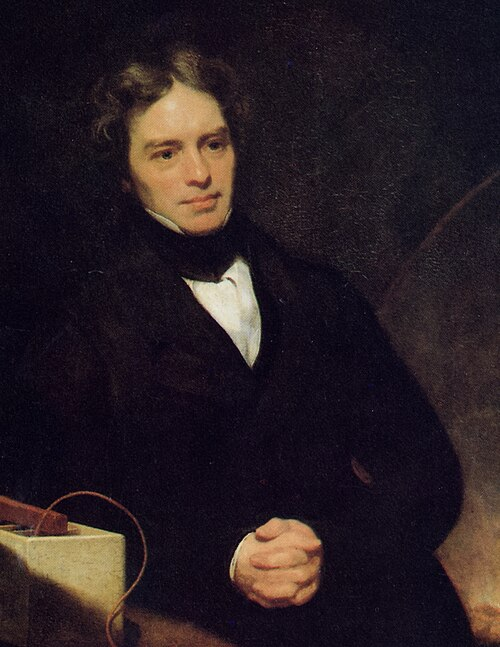
\includegraphics[width=\linewidth]{images/book3/faraday.jpg}
\end{minipage}\hfill
\begin{minipage}[t]{0.69\linewidth}
\vspace{0pt}
1834 में माइकल फ़ैराडे ने, अपनी रचना के एक वोल्टामापी से विद्युत-अपघटनों के उत्पाद
मापते हुए, कहा कि किसी इलेक्ट्रोड पर उत्पन्न पदार्थ का द्रव्यमान
प्रवाहित विद्युत की मात्रा के समानुपाती होता है, और
विद्युत की दी गई मात्रा के लिए भिन्न पदार्थों के द्रव्यमान
उनके रासायनिक तुल्यांकों के अनुपात में होते हैं। उन्होंने इलेक्ट्रोड, ऐनोड, कैथोड,
आयन, ऋणायन और धनायन शब्द गढ़े। उनके नाम वाला स्थिरांक इन नियमों को
$Q = nF\,\Delta\xi$ में बदल देता है। (चित्र: थॉमस फ़िलिप्स,
1842, सार्वजनिक अधिकार-क्षेत्र, विकिमीडिया कॉमन्स।)
\end{minipage}
\end{history}

\section{सांद्रता सेल}

\begin{definition}[सांद्रता सेल]\label{def:b2:cell-thermodynamics:concentration-cell}
\emph{सांद्रता सेल}\index{सांद्रता सेल} एक ही युग्म के दो
अर्ध-सेलों से बना होता है जो केवल किसी एक स्पीशीज़ की सांद्रता (या
दाब) में भिन्न होते हैं।
\end{definition}

\begin{proposition}[सांद्रता सेल की वोल्टता]\label{prop:b2:cell-thermodynamics:concentration-cell}
धातु M के दो इलेक्ट्रोड, जो सांद्रताओं $c_1 < c_2$ वाले \ce{M^{n+}} के
विलयनों में डूबे हों और लवण सेतु से जुड़े हों, यह वोल्टता देते हैं:
\[
  U = \frac{RT}{nF}\ln\frac{c_2}{c_1} ,
\]
धनात्मक ध्रुव अधिक सांद्र पक्ष होता है। सेल तब तक काम करता है जब तक
दोनों सांद्रताएँ बराबर न हो जाएँ।
\end{proposition}

\begin{proof}
नेर्न्स्ट समीकरण से हर इलेक्ट्रोड का $E_i = E^\circ + (RT/nF)\ln c_i$ है (\omterm{def:b2:chemical-potential:ideal-mixture}{आदर्श
तनु विलयन}); अंतर में $E^\circ$ कट जाता है। अभिक्रिया
\ce{M^{n+}}(पक्ष 2) $\to$ \ce{M^{n+}}(पक्ष 1) है: धातु
सांद्र पक्ष (कैथोड) पर जमती है और तनु पक्ष (ऐनोड) पर घुलती है, जो
सांद्रताओं को बराबर करता है; बराबर होने तक $\Delta_r G = RT\ln(c_1/c_2) < 0$
रहता है।
\end{proof}

\begin{omfigure}
\begin{tikzpicture}[font=\small, >={Stealth}]
  \pic at (0,0) {beaker={0.7}{omDef!10}};
  \pic at (3.6,0) {beaker={0.7}{omDef!32}};
  \pic at (-0.3,0.25) {electrode={black!25}};
  \pic at (3.9,0.25) {electrode={black!25}};
  \pic at (0.35,0.55) {saltbridge={2.9}};
  \pic (m) at (1.8,4.3) {meter={V}};
  % common (black) terminal on the anode side, red (+) on the cathode side
  \fill[black] (1.4,4.03) circle (0.065); \fill[red!70!black] (2.2,4.03) circle (0.065);
  \draw[thick] (-0.15,2.65) |- (m-a);
  \draw[thick] (4.05,2.65) |- (m-b);
  \node[anchor=east] at (-0.95,1.0) {\ce{Ag}};
  \node[anchor=west] at (4.45,1.0) {\ce{Ag}};
  \node at (0.25,-0.35) {\ce{Ag+} \qty{0.010}{mol/L}};
  \node at (3.6,-0.35) {\ce{Ag+} \qty{0.10}{mol/L}};
  \node[anchor=east] at (-0.9,2.3) {$-$ ऐनोड};
  \node[anchor=west] at (4.6,2.3) {कैथोड $+$};
  \node[font=\scriptsize] at (-0.1,-0.8) {\ce{Ag -> Ag+ + e-}};
  \node[font=\scriptsize] at (3.7,-0.8) {\ce{Ag+ + e- -> Ag}};
  \node[font=\scriptsize] at (1.8,5.05) {$U = \qty{59}{mV}$};
\end{tikzpicture}

{\small \qty{25}{\degreeCelsius} पर सिल्वर \omterm{def:b2:cell-thermodynamics:concentration-cell}{सांद्रता सेल}। तनु पक्ष
ऐनोड है: वहाँ चाँदी घुलती है और सांद्र पक्ष पर जमती है,
जब तक दोनों सांद्रताएँ बराबर न हो जाएँ। $U = 0.0592\log(0.10/0.010) =
\qty{59}{mV}$।}
\end{omfigure}

यही सिद्धांत सांद्रताएँ मापता है। काँच इलेक्ट्रोड, जिसकी पतली
झिल्ली एक संदर्भ विलयन को नमूने से अलग करती है, \qty{25}{\degreeCelsius} पर
pH अंतर की प्रति इकाई $(RT/F)\ln 10 = \qty{59}{mV}$ का झिल्ली
विभव विकसित करता है: प्रथम वर्ष के खंड का pH मापी \ce{H+} के लिए एक \omterm{def:b2:cell-thermodynamics:concentration-cell}{सांद्रता सेल} है।
किसी जीवित कोशिका की झिल्ली के आर-पार \ce{K+} की असमान सांद्रताएँ
इसी प्रकार कई दसियों मिलीवोल्ट का विभव उत्पन्न करती हैं।

\section{अभ्यास}

\begin{exercise}[$\star$]\label{exo:b2:cell-thermodynamics:1}
$\Delta_f G^\circ(\ce{H2O}, \text{l}) = \qty{-237.14}{kJ/mol}$ से
हाइड्रोजन--ऑक्सीजन सेल की मानक वोल्टता परिकलित कीजिए।
\end{exercise}

\begin{exercise}[$\star$]\label{exo:b2:cell-thermodynamics:2}
एक बैटरी का निर्धारण \qty{1.0}{A.h} है। उसमें संचित आवेश, कूलॉम में,
और पूर्ण अनावेशित होने पर उसके ऐनोड पर उपभुक्त ज़िंक का द्रव्यमान (\ce{Zn -> Zn^2+ + 2e-})
परिकलित कीजिए।
\end{exercise}

\begin{exercise}[$\star$]\label{exo:b2:cell-thermodynamics:3}
एक डेनियल सेल बिना धारा के \qty{1.10}{V} देता है। ज़िंक के एक मोल के लिए $\Delta_r G$
और \qty{10.0}{g} ज़िंक के लिए अधिकतम विद्युत कार्य परिकलित कीजिए।
\end{exercise}

\begin{exercise}[$\star$]\label{exo:b2:cell-thermodynamics:4}
ताँबे के दो इलेक्ट्रोड \qty{1.0e-3}{mol/L} और \qty{0.10}{mol/L} के कॉपर(II) सल्फ़ेट
विलयनों में डूबे हैं। \qty{25}{\degreeCelsius} पर वोल्टता परिकलित कीजिए और
ध्रुवों के नाम बताइए।
\end{exercise}

\begin{exercise}[$\star\star$]\label{exo:b2:cell-thermodynamics:5}
किसी सेल ($n = 2$) के लिए \qty{298}{K} पर $E^\circ = \qty{1.015}{V}$ और $dE^\circ/dT = \qty{-4.0e-4}{V/K}$
है (अभ्यास के आँकड़े)। $\Delta_r G^\circ$, $\Delta_r S^\circ$ और
$\Delta_r H^\circ$ परिकलित कीजिए।
\end{exercise}

\begin{exercise}[$\star\star$]\label{exo:b2:cell-thermodynamics:6}
\cref{exo:b2:cell-thermodynamics:5} का सेल अभिक्रिया के एक मोल का अनावेशन करता है,
(a) उत्क्रमणीय रूप से; (b) \qty{0.90}{V} पर। हर स्थिति में विद्युत कार्य और
परिवेश के साथ विनिमित ऊष्मा परिकलित कीजिए।
\end{exercise}

\begin{exercise}[$\star\star$]\label{exo:b2:cell-thermodynamics:7}
$E^\circ(\ce{Fe^3+}/\ce{Fe})$ को गिब्स संभवन ऊर्जाओं (\ce{Fe^2+} \qty{-78.90}{kJ/mol},
\ce{Fe^3+} \qty{-4.7}{kJ/mol}) से परिकलित कीजिए और जाँचिए कि यह
$(E_1^\circ + 2E_2^\circ)/3$ के बराबर है।
\end{exercise}

\begin{exercise}[$\star\star$]\label{exo:b2:cell-thermodynamics:8}
युग्म \ce{AgCl}/\ce{Ag} का मानक विभव परिकलित कीजिए, फिर
\qty{0.10}{mol/L} पोटैशियम क्लोराइड में डूबे सिल्वर क्लोराइड इलेक्ट्रोड का
विभव।
\end{exercise}

\begin{exercise}[$\star\star$]\label{exo:b2:cell-thermodynamics:9}
ज़िंक--वायु सेल \ce{2Zn + O2 -> 2ZnO} का उपयोग करते हैं ($\Delta_f G^\circ(\ce{ZnO}) =
\qty{-318.30}{kJ/mol}$)। मानक वोल्टता और प्रति किलोग्राम ज़िंक अधिकतम विद्युत
ऊर्जा, \unit{kW.h} में, परिकलित कीजिए।
\end{exercise}

\begin{exercise}[$\star\star\star$]\label{exo:b2:cell-thermodynamics:10}
एक प्रत्यक्ष मेथनॉल ईंधन सेल \ce{CH3OH(l) + 3/2O2 -> CO2 + 2H2O(l)} चलाता है।
$\Delta_f H^\circ$ (\unit{kJ/mol}): \ce{CH3OH(l)} $-239$, \ce{CO2} $-393.51$,
\ce{H2O(l)} $-285.83$; और $S^\circ$ (\unit{J/(K.mol)}): \ce{CH3OH(l)} 127.2,
\ce{CO2} 213.8, \ce{H2O(l)} 69.95, \ce{O2} 205.15 से $n$, $E^\circ$ और
अधिकतम दक्षता परिकलित कीजिए।
\end{exercise}

\begin{exercise}[$\star\star\star$]\label{exo:b2:cell-thermodynamics:11}
किसी सेल ($n = 2$) के लिए \qty{298}{K} पर $E = \qty{0.500}{V}$ और $dE/dT = \qty{+3.0e-4}{V/K}$
है (अभ्यास के आँकड़े)। दिखाइए कि उत्क्रमणीय रूप से काम करते हुए वह
$-\Delta_r H$ से अधिक विद्युत कार्य देता है, और समझाइए कि अतिरिक्त ऊर्जा कहाँ से आती है।
\end{exercise}

\begin{exercise}[$\star\star\star$]\label{exo:b2:cell-thermodynamics:12}
दो हाइड्रोजन इलेक्ट्रोड (\ce{H2} के \qty{1}{bar}) pH 7.00 वाले एक संदर्भ विलयन
में और एक नमूने में डूबे हैं। \qty{25}{\degreeCelsius} पर वोल्टता \qty{0.177}{V} है,
संदर्भ धनात्मक ध्रुव है। नमूने का pH ज्ञात कीजिए, और समझाइए
कि परिणाम किसी मानक विभव पर निर्भर क्यों नहीं करता।
\end{exercise}

\section{समस्या: ईंधन-सेल बस}

\begin{problem}[{सप्ताहांत समस्या --- गिब्स ऊर्जाओं से
हाइड्रोजन--ऑक्सीजन सेल की मानक वोल्टता, उसका ताप गुणांक, किसी वास्तविक पुंज की
दक्षता और ऊष्मा, और हाइड्रोजन की एक टंकी में ऊर्जा}]
\label{pb:b2:cell-thermodynamics:1}
एक ईंधन-सेल पुंज में श्रेणी में 400 सेल हैं, हर एक में प्रोटॉन-विनिमय
झिल्ली (अम्लीय विद्युत-अपघट्य)। \qty{298.15}{K} पर आँकड़े (CODATA, JANAF):
$\Delta_f H^\circ(\ce{H2O}, \text{l}) = \qty{-285.83}{kJ/mol}$, $\Delta_f
G^\circ(\ce{H2O}, \text{l}) = \qty{-237.14}{kJ/mol}$, $\Delta_f G^\circ(\ce{H2O},
\text{g}) = \qty{-228.58}{kJ/mol}$; $S^\circ$ (\unit{J/(K.mol)}): \ce{H2O(l)} 69.95,
\ce{H2} 130.68, \ce{O2} 205.15। $F = \qty{96485}{C/mol}$; $M(\ce{H2}) =
\qty{2.016}{g/mol}$।
% ledger: dfh:H2O-l, janafG:H2O_l.298, janafG:H2O.298, s0:H2O_l, s0:H2_g, s0:O2_g, const:F, aw:H

\medskip
\noindent\textbf{भाग I --- मानक वोल्टता।}
\begin{enumerate}
  \item ऐनोड और कैथोड पर अर्ध-अभिक्रियाएँ, और सेल
        अभिक्रिया लिखिए।
  \item हाइड्रोजन के प्रति अणु कितने इलेक्ट्रॉन विनिमित होते हैं?
  \item जल के द्रव रूप में बनने पर $E^\circ$ परिकलित कीजिए।
  \item जल के वाष्प रूप में निकलने पर इसे परिकलित कीजिए।
  \item जल के वाष्पन की \omterm{def:b2:reaction-free-energy:gibbs-energy}{गिब्स ऊर्जा} से अंतर समझाइए।
  \item \qty{298}{K} पर $\Delta_r H^\circ$ और अधिकतम दक्षता परिकलित कीजिए।
\end{enumerate}

\medskip
\noindent\textbf{भाग II --- ताप।}
\begin{enumerate}[resume]
  \item द्रव जल के लिए $\Delta_r S^\circ$ परिकलित कीजिए।
  \item $dE^\circ/dT$ निकालिए।
  \item पुंज के कार्य-ताप, \qty{80}{\degreeCelsius}, पर $E^\circ$ का
        आकलन कीजिए।
  \item अपनी विधि की तुलना \qty{400}{K} पर JANAF मान, $\Delta_f
        G^\circ(\ce{H2O}, \text{l}) = \qty{-221.01}{kJ/mol}$, से कीजिए।
  \item \qty{298}{K} पर उत्क्रमणीय सेल प्रति मोल हाइड्रोजन कितनी ऊष्मा का विनिमय करता है?
        वह प्राप्त होती है या मुक्त?
  \item \qty{80}{\degreeCelsius} पर अधिकतम दक्षता का आकलन कीजिए।
\end{enumerate}

\medskip
\noindent\textbf{भाग III --- प्रति सेल \qty{0.70}{V} पर वास्तविक पुंज।}
\begin{enumerate}[resume]
  \item प्रति मोल हाइड्रोजन विद्युत कार्य परिकलित कीजिए।
  \item $\Delta_r H^\circ$ और $\Delta_r G^\circ$ के सापेक्ष दक्षता परिकलित कीजिए।
  \item प्रति मोल हाइड्रोजन मुक्त ऊष्मा परिकलित कीजिए।
  \item इसका कितना भाग अपरिहार्य है, और कितना धारा के कारण?
  \item पुंज \qty{300}{A} देता है। एक सेल की, फिर पुंज की, हाइड्रोजन खपत,
        मोल और ग्राम प्रति सेकंड में, परिकलित कीजिए।
  \item पुंज की विद्युत शक्ति परिकलित कीजिए।
  \item शीतलन परिपथ द्वारा हटाई जाने वाली ऊष्मा शक्ति परिकलित कीजिए।
\end{enumerate}

\medskip
\noindent\textbf{भाग IV --- टंकी।}
\begin{enumerate}[resume]
  \item \qty{5.0}{kg} में हाइड्रोजन की कितनी मात्रा है?
  \item इस हाइड्रोजन के ऑक्सीकृत होने पर सभी सेलों पर गिनकर
        कितना आवेश सेलों से गुज़रता है?
  \item प्रति सेल \qty{0.70}{V} के साथ पुंज द्वारा दी गई विद्युत ऊर्जा
        परिकलित कीजिए।
  \item इसे किलोवाट-घंटों में बदलिए।
  \item पुंज प्रश्न 18 की अपनी शक्ति कितनी देर तक दे सकता है?
  \item प्रति सेल \qty{0.70}{V} पर \qty{5.0}{kg} हाइड्रोजन द्वारा दी गई विद्युत ऊर्जा
        बताइए।
\end{enumerate}
\end{problem}
